\documentclass{article}
\usepackage[T1]{fontenc}
\usepackage{lmodern}
\usepackage{graphicx}
\usepackage{amsmath,amssymb}
\usepackage[a4paper,margin=2cm]{geometry}
\usepackage[absolute,overlay]{textpos}
\setlength{\TPHorizModule}{1mm}
\setlength{\TPVertModule}{1mm}
\usepackage[indonesian]{babel}
\usepackage{hyperref}
\setlength{\emergencystretch}{2em}
% unit: Halaman 35

\begin{document}

% === Halaman 35 (llm) ===

Cek video TUTORIAL CARA MENGGUNAKAN WIRESHARK | MENEMUKAN U53RN4M3 P455WORD PADA LALU LINTAS PACKET JARINGAN:\newline\url{https://www.youtube.com/watch?v=HMkIhUEByd4}

\vspace{70mm}

TUTORIAL CARA MENGGUNAKAN WIRESHARK | MENEMUKAN U53RN4M3 P455WORD PADA LALU LINTAS PACKET JARINGAN

% deskripsi: Screenshot tampilan layar browser yang menampilkan video tutorial YouTube mengenai penggunaan Wireshark untuk memonitoring jaringan dan analisis paket data.
% bbox normalisasi: [0.1400, 0.2100, 0.7400, 0.8900]
\begin{textblock*}{126.00mm}(29.40mm,62.37mm)
\noindent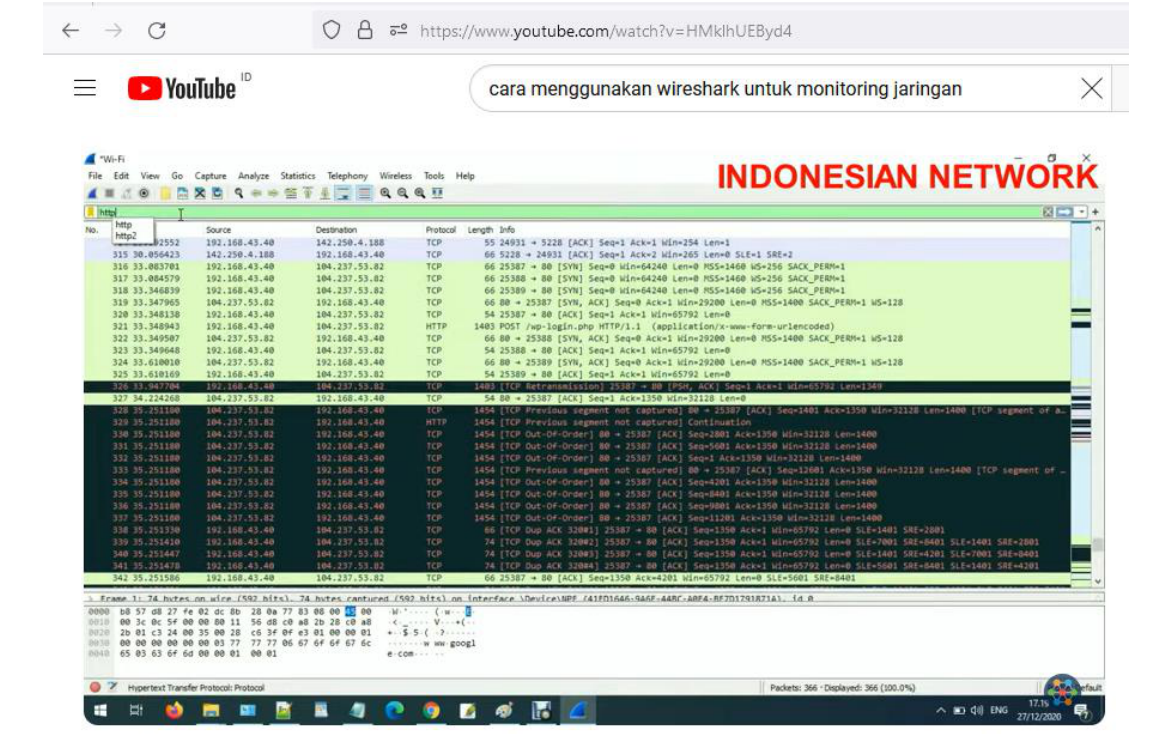
\includegraphics[width=126.00mm,height=201.96mm]{../../images/llm/page_035_img_01.png}%
\end{textblock*}

\end{document}
